% Let's start this by talking right away about changes rather than just ASTs
The general idea for automatically finding the pervasive code patterns within a list of programs is to parse the programs and encode the important parts of the derived AST in fixed-size datapoints. We need fixed-size datapoints, as it is a requirement for both centroid-based and density-based well-known clustering algorithms. Work in this vein makes the assumption that each cluster corresponds to one change pattern.

Our pipeline for finding pervasive patterns in Rust programs also follows this idea. We decided to implement our pipeline completely in Python. To make this work, we need a way to get an AST as a Python dictionary. Syn\footnote{\url{https://crates.io/crates/syn}} is a Rust crate which aims to serve Rust procedural macros. However, it includes a parser which is suitable for our purposes; we simply had to write a preprocessor to transform Syn AST output into Python dictionaries.

% TODO Define change
A change pattern categorizes a class of changes. We thus need to define what a change is. For our purposes, a change is ....
To compute the contents of a change, we need two code revisions: the revision before the commit, and the revision after it. After parsing these two revisions, we will have two ASTs, encoded in two Python dictionaries. Tree diff algorithms can compute the differences between two arbitrary trees. If the trees are programs' abstract syntax trees, we call their diff an ASTDiff. We use dictdiff to obtain ASTDiffs.

An ASTDiff may include an arbitrary number of semantic changes, although a best practice is to include only one semantic change in a commit. Because that best practice is not universally followed, we are interested in finding the most important change within an ASTDiff, and encoding that change in our datapoints. Sections~\ref{sec:path_extraction}~and~\ref{sec:weighting_scheme} provide a detailed explanation of how we select the most important semantic information, which then allowed us to obtain clusters that contained similar datapoints. 

Our target repositories were the top 18 most-starred open source Rust projects on GitHub. Using Pydriller, a repository miner for Python, we mined all the bug related commits and ran them through our pipeline. Then, we applied the DBSCAN clustering algorithm on the resulting datapoints. In Section~\ref{sec:clustering_data} we justify our choice of DBSCAN for clustering, and how we tuned it to improve cluster quality. 

\subsection{\label{sec:data_modelling}Data modelling}

\subsubsection{\label{sec:parsing_programs}Parsing Programs}

% TODO: BCL elements goes in an appendix.
As mentioned above, we use Syn for parsing Rust. Syn handles all of Rust. Each of our datapoints specifies whether any Syn non terminal (\texttt{NT}) is present or absent, i.e. containing one dimension per non terminal. However, we are also interested in change patterns that involve the borrow checker (BC), so we also add a dimension reflecting the presence of a set of BC-related lexemes (BCL) that we identified, e.g. \texttt{clone}, \texttt{Rc}, \texttt{Box}. The full list of \verb+BCL+ elements can be found within our artifact. 
% I think we don't need this sentence here. Let's see what we do later.
%We define dimension items as \verb+DI = NT+ $\cup$ \verb+BCL+, as this set also equals the columns of our tables.

We parse two versions of a changed Rust file in a commit: the file before the commit and after it. This yields two Syn trees. Using the PLY tool (a Python implementation of lex and yacc), we wrote a simple transformer from the serialized Rust AST to Python dictionaries. The change that transforms the first tree to the second one is the fix that was applied in the commit. To find this difference, we use dictdiff, a Python library to find the diff of two Python dictionaries. Its output, in our context, is the ASTDiff.

An ASTDiff, as computed by dictdiff, contains a type:
\begin{itemize}
\item `add': A new structure has been added to the tree; 
\item `remove': A structure has been dropped from the tree; 
\item `change': The content of a sub structure of the first tree has changed.
\end{itemize}
% the description of the context in 2.1.2 is probably enough, you don't need it here, just remove it. I think that you just put the above itemize into 2.1.2 and erase the next paragraph, unless you can spot something you need to add to 2.1.2.
It also encodes the context of the modification. This context happens to be the root elements in our file, e.g. function blocks, struct blocks, impl blocks, etc. The modified content within a context is still in the form of tree. Our objective right now is to find primary elements in our diff that describe the semantics of occurred change.
% TODO rework the above paragraph

\subsubsection{\label{sec:path_extraction}Path Extraction}

\begin{figure}[h]
\centering
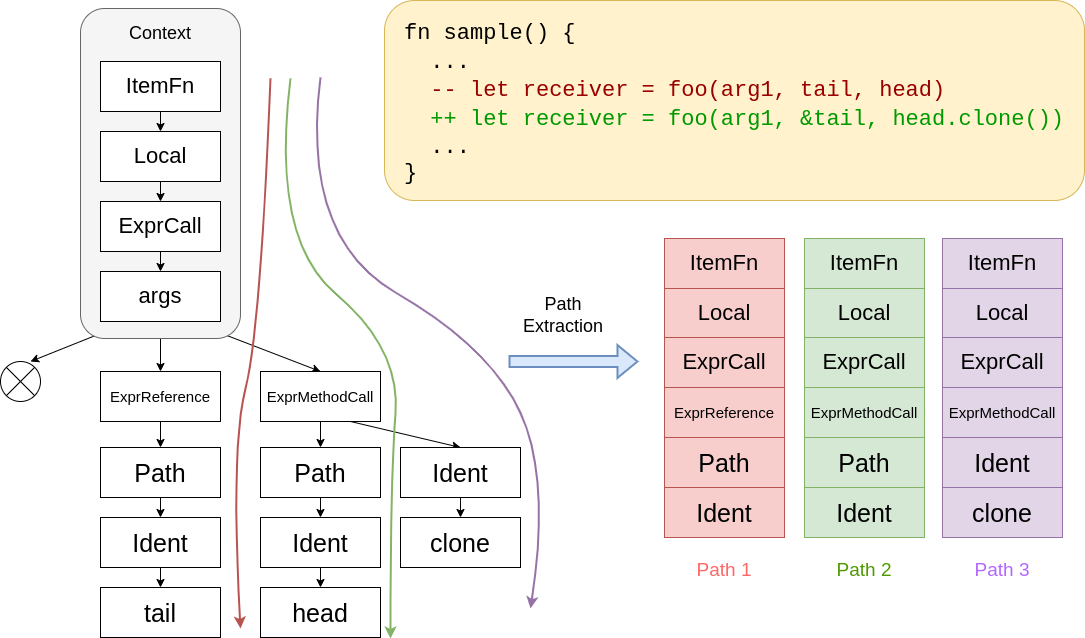
\includegraphics[width=0.8\textwidth]{figs/extraction.png}
\caption{\label{fig:extraction}Path Extraction}
\end{figure}

% remove redundancy between the description of the ASTDiff in 2.1.1 and what we have here. Probably it can go all into 2.1.2, i.e. you can just move the last para of 2.1.1 to here and incorporate it.
The output of dictdiff is a list of diffs, where each diff comprises three parts. The first part specifies whether the modification is of type `add', `remove', or `change'. The second part identifies the context of the modification, that is, the path from the root of the tree to the subtree in which the modification has occured. The third part is the content of the change (terminals and nonterminals). Our tool looks for changes within each root-level scope. That is, our assumption is that a change pattern occurs within one root-level scope. In this work, we chose to not handle patterns that involve changes in multiple functions or multiple files. However, our tool would detect both continuous and non-continuous line changes within one scope.
% TODO provide an example and then transform it into fig:extraction. 

Looking at the tree encoded in the content part of each diff, we realized that each path to a leaf represents one contributing element to the change. A Depth First Search allows us to collect all paths, and we return only the paths that we store in our datapoints (i.e. touching $\mathtt{NT} \cup \mathtt{BCL}$).

Figure~\ref{fig:extraction} illustrates path extraction on a simple change. The change replaces \verb+tail+ with \verb+&tail+ and \verb+head+ with \verb+head.clone()+. That is, after the change, the second argument passes a borrow of \verb+tail+ rather than sending the ownership of \verb+tail+ to the callee; and, in the third argument, instead of sending \verb+head+ to the callee, it sends a clone of it. A DFS on this tree yields three different paths, which we show in red, green, and purple. A path represents a sequence of involved non terminals. We found it crucial to record the order of nodes in the path, as this gives us the freedom to later record the order in our datapoint encoding.

% I think I would move the discussion of why fixed size from the beginning of the section to here; we don't need it at the beginning of the section.
% I think it would be better to show an example of the two if statements either way
\paragraph{Encoding the data.} A key question is how to transform these paths to a fixed size datapoint. First, we need to define a fixed set of columns. The number of columns would depend on the amount of information we want to encode in the datapoints. The most naive approach would be to only report the observed non terminals within the diff. That yields a fully order-insensitive representation. In such an encoding, for instance, there is no difference between two nested if statements and two if statements beside each other. On the other hand, theoretically, for full order-sensitiveness, we would need to encode all possible combinations of items from $\mathtt{NT} \cup \mathtt{BCL}$ as our dimensions, which yields an infeasible $O(n^n)$ dimensions; this could potentially be reduced somewhat, but is still impractical. A reasonable work around would be to reduce $n$ from the full set of non terminals to a smaller set of categories (e.g. a category for larger entites like class or function definitions, and a category for smaller entities like statements and expressions), and then to record all possible combinations of these categories (similar to JS authors~\cite{foo}). That approach reduces the number of dimensions and provides more reasonable and syntactically-correct combinations. However, it would still yield a sparse dataset. 
% todo you need to dig up the JS paper ref

% ok, add a figure and then we'll look at the text again and follow along with the picture
In our methodology, we propose a novel representation. Similar to the first approach, we order-insensitively define the columns of our dataset as the set of items $\mathtt{NT} \cup \mathtt{BCL}$ we collected from Syn. However, to simulate order-sensitiveness, we carried out two auxiliary steps. First, we record the number of occurrences of items within the paths at each scope. The reason behind this decision is because a different order of program elements yields a different number of occurrences of underlying dimension items. Second, we semi-automatically design a weighting scheme to prioritize non terminals that we think are more salient for Rust bugs.

\subsubsection{\label{sec:weighting_scheme}Weighting Scheme}

Our main requirement is that our datapoints summarize the key changes in ASTDiffs---a datapoint should foreground the most important change in a diff. For instance, the purple (right-most) path in Figure~\ref{fig:extraction} could be described as a change in a local variable declaration; a change in a function call; calling a method of one of the function arguments; or calling clone() on one of the function arguments. The last description is the most useful one, and we designed our weighting scheme to encode this value judgment.

We made two observations about changes. First, we saw that an item (non terminal or BC-related lexeme) that occurs closer to AST leaves tends to be more semantically important. Relatedly, items closer to the root tend to be repeated in all the paths within one ASTDiff (e.g. ItemFn, Local, ExprCall in Figure~\ref{fig:extraction}). We thus want to prioritize items that tend to occur closer to leaves and de-prioritize items that tend to occur closer to roots.

To design our weighting scheme, we collected empirical data about locations of item occurrences in a corpus. Specifically, we mined the last 20 bug related commits of the last 20 most-starred Rust projects on GitHub, and ran them through our pipeline. We recorded the total number of occurrences of each item. Then, if $\# i$ is the number of occurences of $i$, we gave $i$ a weight of $1/\# i$. Because items that occur closer to the root also occur more often, per our observation, this gives higher weights to items that occur infrequently, i.e. closer to the leaves. Items that occur often and have lower weights are, we believe, less important in describing a change.

Furthermore, as we wanted to make sure that our tool captures patterns related to the Rust borrow checker, we manually increased the weights of the \texttt{BCL} items. The manual adjustment is why we characterize our weighting scheme as semi-automatically designed. 

\subsection{\label{sec:mining_repositories}Mining Repositories}

\begin{figure}[h]
\centering
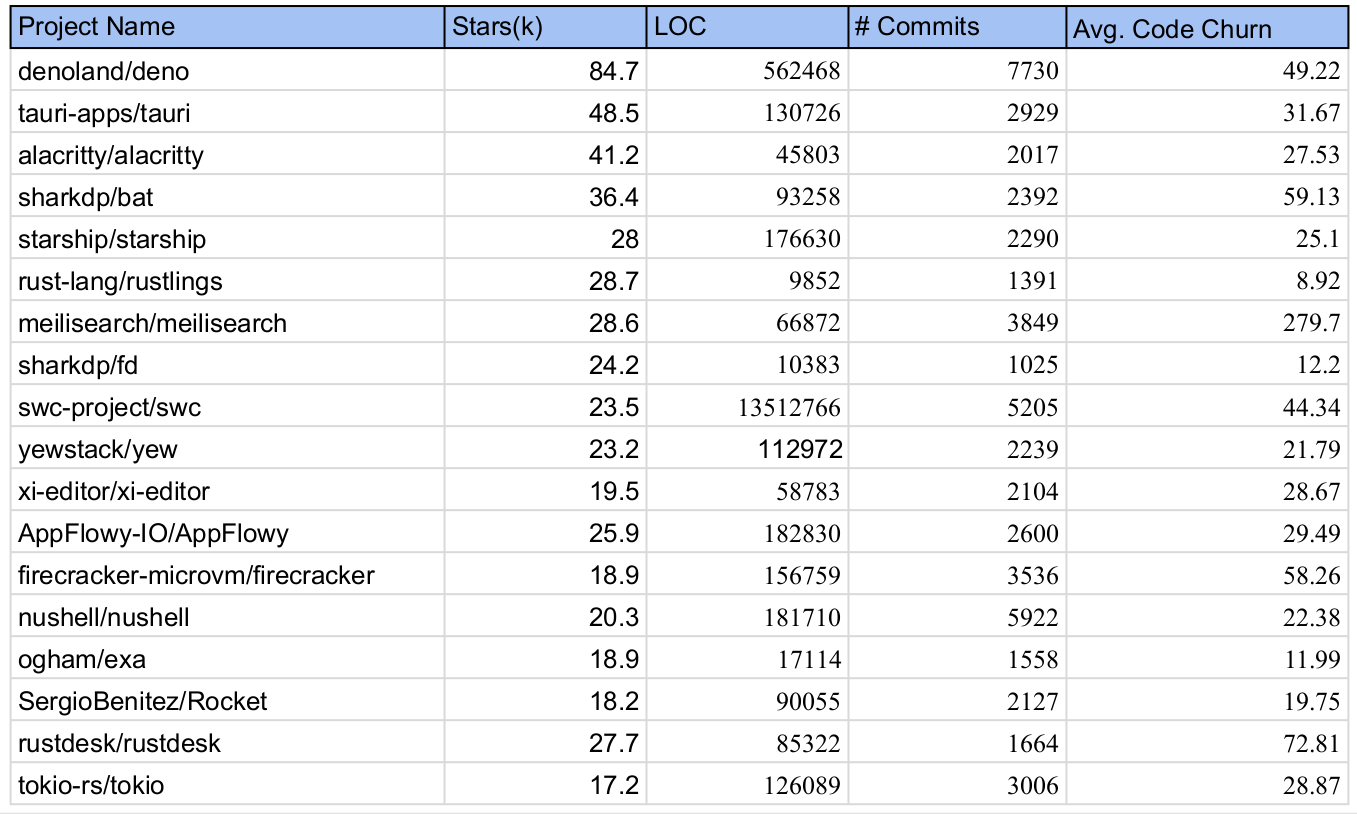
\includegraphics[width=1\textwidth]{figs/repos.png}
\caption{\label{table:repos} Target Repositories}
\end{figure}

Now that we have set up our code analysis pipeline, we can start mining the Rust repositories. We target the top 18 most starred Rust projects on GitHub, at the time of data collection. The details of these projects are outlined in Table \ref{table:repos}. We computed the average code churn of the files within the projects. denoland/deno and swc-project/swc are the projects with largest number of LOCs and average code churn. Unsurprisingly, we captured a lot of instances from these two projects in our final clusters.

We use Pydriller, a Python library for mining software repositories. Pydriller provides APIs to extract commits from a Git repository, and search through different revisions of files. Algorithm \ref{alg} shows how we leveraged Pydriller to run the target repositories through our code analysis pipeline, and populate two databases; one for general patterns and one for borrow-checker related patterns. The borrow-checker related patterns are the changes that include certain keywords (e.g. clone, Box, etc. Full list can be found in our artifact). For each repository, we search through all the commits that include bug fixing related keywords within their commit messages. These keyword for the scope of our project are `bug', `error', `fault', `defect', and `fix'. 

Next, we collect a pair of revision per each Rust file. The pair includes the state of the file before commit and after commit ($f_a, f_b$). After parsing each revision and computing the ASTDiff, we can obtain the fixed sized datapoint $DP$. If the datapoint contains borrow-checker related keywords, we would put that inside the BC-related code changes table ($D_b$), otherwise we would put it in the general code changes table ($D_g$). In both cases, we augment the datapoint with the commit hash, filename, and the scope in which the change has happened. In case of BC-related code changes, we also store detected BC-related keyword. Now our tables are ready for clustering and categorization.

\begin{algorithm}
\caption{\label{alg} Mining Algorithm}
\hspace*{2mm} \textbf{Input:} $R$ (target repositories)  \\
\hspace*{2mm} \textbf{Output:} $D_g$ (General code changes) \\
\hspace*{2mm} \textbf{Output:} $D_b$ (BC-related code changes)
\begin{algorithmic}
\State $D_g \leftarrow \phi$
\State $D_b \leftarrow \phi$
\For{$r \in R$}
    \For{$c \in \textsc{ExtractCommits}(r)$}
        \If{$c.msg$ contains bug fixing related keywords}
            \For{$\{f_b, f_a\} \in \textsc{GetModifiedRustFiles}(c)$}
                \For{$e \in \textsc{ASTDiff}(\textsc{Parse}(f_b), \textsc{Parse}(f_a))$}
                    \State $DP \leftarrow \textsc{GetDataPoint}(e)$
                    \State $DP \leftarrow c.hash \cup f_a.name \cup e.scope \cup DP $
                    \If{$\textsc{IsBCRelated}(e)$}
                        \State $DP \leftarrow \textsc{GetBCKeyword}(e) \cup DP $
                        \State $D_b \leftarrow D_b \cup DP$
                    \Else
                        \State $D_g \leftarrow D_g \cup DP$
                    \EndIf
                \EndFor
            \EndFor
        \EndIf
    \EndFor
\EndFor
\end{algorithmic}
\end{algorithm}

\subsection{\label{sec:clustering_data}Clustering Data}

We use DBSCAN clustering algorithm for two main reasons. Firstly, it is a density-based clustering method, which means that it detects arbitrarily shaped clusters as opposed to centroid-based methods, like k-means. Secondly, also in contrast to k-means, it does not require the number of clusters in advance as an input to the algorithm.

There are two parameters that need tuning in DBSCAN. First parameter is $\epsilon$ which indicates a radius with which you can decide whether a point is a core point, a border point, or an outlier. Second parameter is the minimum number of point you would like each cluster to have. We denote his parameter with $Z$. We ran DBSCAN using different combinations of these two parameters. In Figure \ref{fig:clustering}, we show nine different experiments with their respective parameter values. Within each subplot, the number of clustered points, noise points, and the number of clusters have been specified both for $D_g$ and $D_b$. 


\begin{figure}[h]
\centering
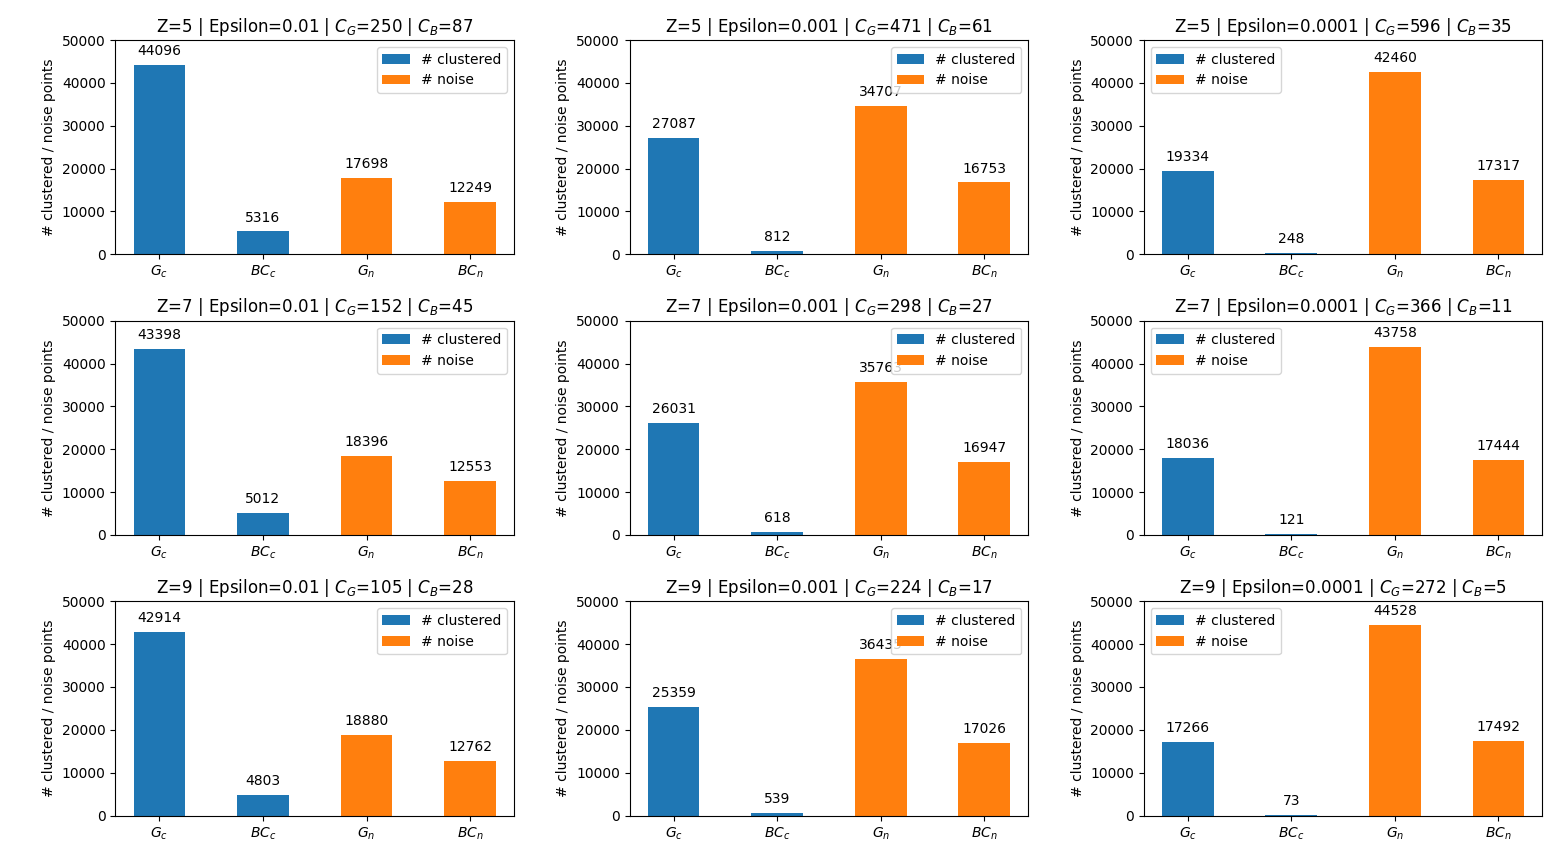
\includegraphics[width=1\textwidth]{figs/clusters.png}
\caption{\label{fig:clustering} Clustering Experiments}
\end{figure}

As a general rule, a lower value for $Z$ would allow more group of close points to be considered as clusters, resulting in a higher number of clusters. A large value for $\epsilon$ would widen the search radius, allowing more points to fall in the clusters which results in a reduction of the number of noise points. That possibly can put points that do not completely manifest same patterns inside a cluster, resulting in a ineffective clustering. Alternatively, a small value for $\epsilon$ would tighten the ring of search, possibly separating clusters which essentially manifest same code changes. Also if $\epsilon$ is really small, the clustering algorithm might not detect some clusters at all, resulting in a reduction of the number of clusters. 

\subsubsection{\label{sec:manual_analysis_parameter_tuning}Manual Analysis for parameter tuning}

That is why, we carried out a manual analysis of clusters. In the manual analysis we randomly pick 50 clusters and from each cluster we randomly choose 10 datapoints. The analyzer then looks at the code and specify the clusters that contained more than five datapoints showing similar patterns. Through the manual analysis we specified that $\epsilon=0.0001, Z=5$ and $\epsilon=0.001, Z=5$ acted as the best parameters for $D_g$ and $D_b$, resulting in 596 and 61 clusters, respectively. As the final step, we exclude the clusters that contained datapoints from less than 3 projects. That is because, we wanted our clusters to contain cross-project patterns as much as possible.  

\subsubsection{\label{sec:manual_analysis_cluster_selection}Manual Analysis for cluster selection}
% 3 types, refactoring dropped

Similar to ..., following Cotroneo et al. definitions, we divide the clusters in three different groups:

\begin{itemize}
    \item bug-fix: "The changed code actually fixes the behavior of software, which can represent fixes for a bug type". We consider the changes that improve program performance as instance of this group, as they fix the behavior of software.
    
    \item fix-induced: "The changed code is a group of bug-fixing code changes but not represents an actual bug fix, e.g., adding new input parameters to a method, the method signature and method call must be changed corresponding".
    
    \item refactoring: "the changed code does not modify the software behavior, e.g., better readability or encapsulation".
\end{itemize}

In this work, we were only interested in the first two group and disregarded the the clusters that manifest a refactoring change. Also, we prefer reporting clusters that manifest concrete patterns. An abstract pattern as opposed to a concrete pattern can account for many changes in the programs. For instance, the pattern `Adding a new statement to a function's body' is deemed more abstract than `Changing a clone of a variable to a borrowing of it in a function argument'.

In our manual analysis, we randomly picked 50 datapoints of each cluster. If the cluster had less than 50 datapoints, we would analyze all of the datapoints in the cluster. Next, we read the code and also the bug report related to all the datapoints (if existed). In case that a similar pattern was detected over the instances of a cluster, we would write a natural language description of that cluster. After providing all the descriptions, we linked similar clusters together as possible candidates for merging. At last, after accomplishing re-examination for merge possibilities, we selected 19 clusters that manifested concrete changes. We discuss about our findings in Section \ref{sec:common_patterns} and \ref{sec:bc_patterns}.




